\chapter{Applications of Machine Learning}

Machine learning is becoming more and more integrated in our daily lives. For e.g. \textbf{Google} uses machine learning extensively to detect our search patterns and show us the results we want to see in our daily lives. 

\begin{wrapfigure}{r}{0.6\textwidth}
\vspace{-25pt}
  \begin{center}
    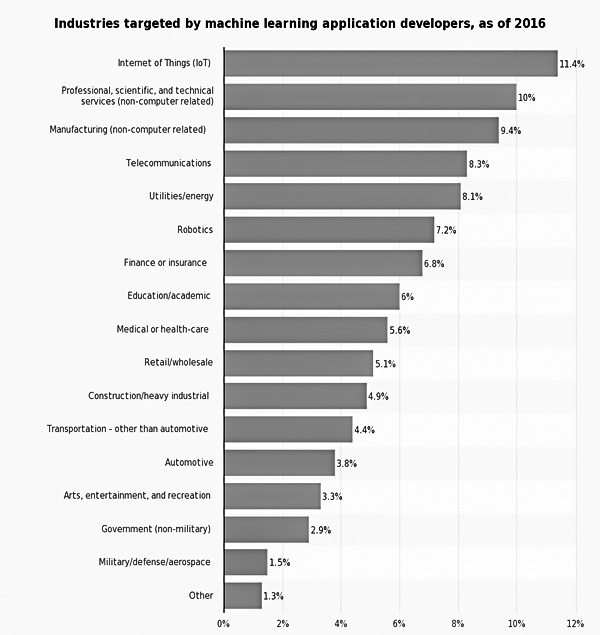
\includegraphics[width=0.58\textwidth]{machine_learning_target.jpg}
  \end{center}
  \vspace{-30pt}
  \caption{The top industries focusing on applying machine learning, including Internet of Things (IoT), professional/scientific/technical services (non-computer related), manufacturing, telecommunications and utilities/energy, according to a report by Forbes in June 2016.}
  \vspace{-30pt}
\end{wrapfigure}

It is true that a person's habits or maybe even character can be determined or deduced by going through the internet history, search patterns and companies make business out of it.
\section{Social Media Applications}
The first industry to accept machine learning to make people's lives easier was \textbf{Social Media}. It is ever growing and now an integral part of our lives.
Every single bigheads and small-heads in the social media industry has an R\&D Department to develop new algorithms of machine learning which will attract more and more people to their websites and make people more attracted to social media.
\begin{description}
	\item[Twitter :]
	Twitter uses machine learning to spread the reach organically, even if the reach is considered very less in twitter. Almost an year ago \textbf{Jack Dorsey}, CEO and Founding member of \textbf{twitter} said this in an announcement ---
	\begin{quotation}
		Magic Pony’s technology – based on research by the team to create algorithms that can understand the features of imagery – will be used to enhance our strength in live and video and opens up a whole lot of exciting creative possibilities for Twitter. The team includes 11 PhD-s with expertise across computer vision, machine learning, high-performance computing, and computational neuroscience, who are alumni of some of the top labs in the world.
		
		We are continuing to build strength into our deep learning teams with world-class talent to help Twitter be the best place to see what’s happening and why it matters, first. We value deep learning research to help make our world better, and we will keep doing our part to share our work and learning with the community.
	\end{quotation}
	\item[Facebook:]
	Machine learning is essential to \textbf{Facebook}. It helps people discover new content and connect with the stories they care the most about. \textbf{Facebook}'s  machine learning algorithms rank feeds, ads and search results, and create new text understanding algorithms that keep spam and misleading content at bay. New computer vision algorithms can “read” images and videos to the blind and display over 2 billion translated stories every day, speech recognition systems automatically caption the videos that play in our news feed, and helps create new magical visual experiences such as turning panorama photos into fully interactive 360 photos.
	\begin{quote}
	 “We seek to advance the state of the art in machine learning for maximum impact, and our efforts form the glue between science and research and Facebook experiences.”
	 ---  \textit{Joaquin Quinonero Candela, Director of Applied Machine Learning}
	\end{quote}
	\textbf{Facebook}'s machine learning usage is one of the biggest in all the industries worldwide. It facilitates around 1.74 billion people everyday all over the world in a way that was unthinkable even two years back.
\end{description}
While these two are the big players in the social media industry, machine learning is used in almost everywhere in the internet and all of the services that are owned by \textbf{Google}. One of the largest machine learning frameworks, \textbf{\textit{TensorFlow}} is owned, developed and used by \textbf{Google} everyday.
\section{Medical Usages of Machine Learning}
One of the fields where machine learning is being used extensively besides \textbf{Social Media} is the \textbf{Healthcare} field. A very important and very promising side is opened by the usage of machine learning in the \textbf{Healthcare} industry.
\subsection{Oncology}
Over the past decades, a continuous evolution related to cancer research has been performed\cite{hanhen11}. Scientists applied different methods, such as screening in early stage, in order to find types of cancer before they cause symptoms. Moreover, they have developed new strategies for the early prediction of cancer treatment outcome. With the advent of new technologies in the field of medicine, large amounts of cancer data have been collected and are available to the medical research community. However, the accurate prediction of a disease outcome is one of the most interesting and challenging tasks for physicians. As a result, ML\footnote{Machine Learning} methods have become a popular tool for medical researchers\cite{cicchetti92}. These techniques can discover and identify patterns and relationships between them, from complex datasets, while they are able to effectively predict future outcomes of a cancer type.
\begin{figure}
\centering
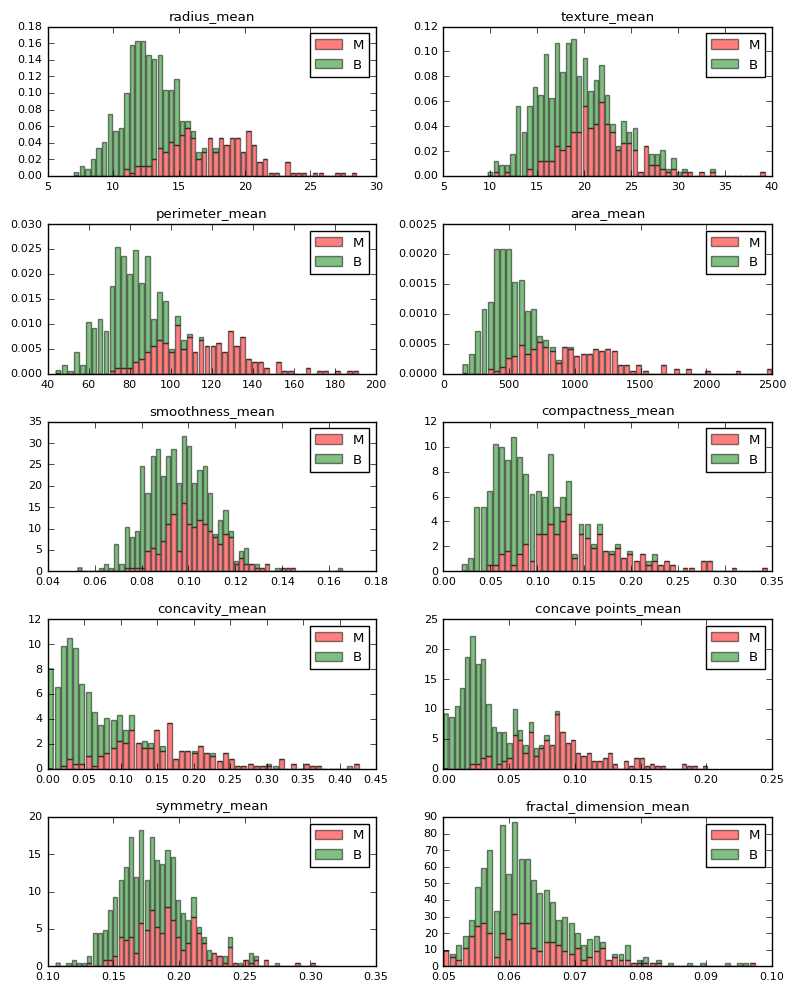
\includegraphics[scale = 0.55]{cancer}
\caption{A machine learning report of Breast Cancer Prediction from a dataset.\cite{kagglecancer}}
\end{figure}
\begin{description}
	\item[Diagnosis :]
	According to an article in \textbf{Forbes} magazine on September, 2016, 22 big companies in medical industry are developing new programs for imaging and diagnostics using machine learning. However, the news doesn't stop here, it also cites that a group named \textbf{Pathway Genomics}, backed by \textbf{IBM}, a leader in computer industry is developing a simple blood test algorithm to determine if early detection of certain types of cancer is possible
	
	Another one of the pioneers in the industry, \textbf{Lumiata} has developed predictive analytics tools that can discover accurate insights and make predictions related to symptoms, diagnoses, procedures, and medications for individual patients or patient groups.
	\item[Treatment :]
	\textbf{IBM}'s \textbf{Watson}, a cognitive R\&D Dept. has been tasked with helping oncologist make decisions about patients and develop a system which will determine what is the best for each and every patient. The program is named \textbf{CareTrio} as it combines three packages, \textit{CareEdit}, which helps create documentation of cancer treatment more easy for the doctors so that references can be used. \textit{CareGuide}, is a \emph{"clinical guide support system"} which analyses the data of CareEdit and supports the doctors in making a decision.  \textit{CareView} is an analysis tool that can evaluate the outcome of past clinical decisions and identify patients who received different treatments than the recommendations. This kind of retrospective can help doctors refine their guidelines, closing the circle back to the CareEdit tool.
\end{description}
\subsection{Other than Oncology}
But the advances don’t stop with diagnosis or treatment. One of the biggest hurdles in health care is hospital re-admittance. Doctors around the world struggle with how to keep their patients healthy and following their treatment recommendations when they go home.

\textbf{AiCure} is using mobile technology and facial recognition technologies to determine if a patient is taking the right medications at the right time to help doctors confirm that the patient is taking their medications and alert them if something goes wrong.

\textbf{NextIT} is developing a digital health coach, similar to a virtual customer service rep on an e-commerce site. The assistant can prompt questions about the patient’s medications and remind them to take the medicine, ask them about symptoms, and convey that information to the doctor.

\textbf{The Caféwell Concierge} app uses IBM’s Watson’s natural language processing (NLP) to understand users health and wellness goals and then devise and provide the right balance of nudges and alerts so users can meet their targets and the app can reward them.

Figure 3.3 shows some features of McDonald's food healthiness from a machine learning experimentation with open datasets\cite{macd}.
\begin{figure}
\centering
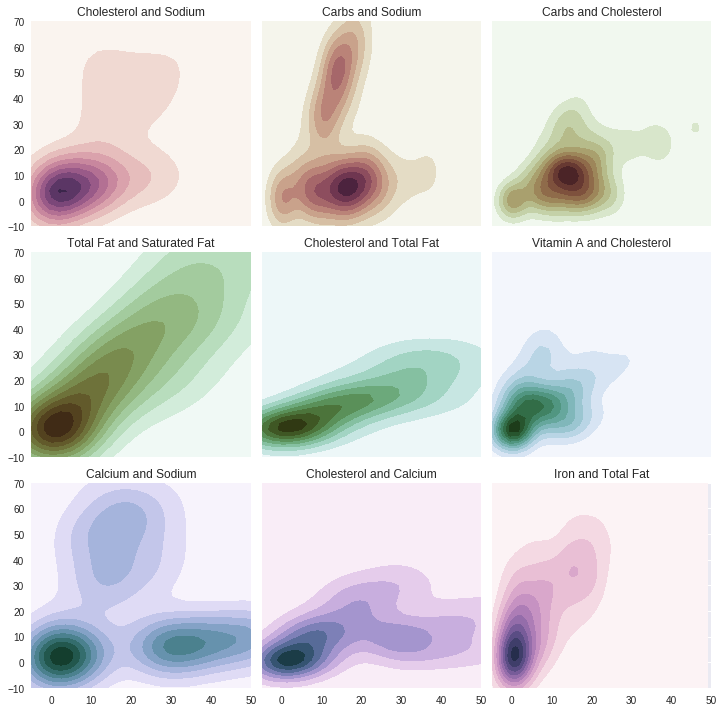
\includegraphics[scale=0.5]{mcd}
\caption{Comparisons of Features via Contour and Correlation plots}
\end{figure}

And this is just the beginning.  As these technologies develop, new and improved treatments and diagnoses will save more lives and cure more diseases. The future of medicine is based in machine learning.